Consider the eigenvalue problem for the 2D Laplacian on the domain $\Omega \in [0, 1] \times [0, 1]$ with Dirichlet
boundary conditions:

$$
\Delta u = \lambda u
$$

Solve for $u$ using the 5-point Laplacian and explain how well the eigenvalues $\lambda_{m,n} = -(m^2 + n^2)\pi^2$ are
approximated. Plot eigenfunctions for the first few eigenvalues.

\begin{solution}\ \\\\
    \ \\
    \newpage

    \noindent The first four eigenvalues (with $(m, n) \in [1, 2] \times [1, 2]$ with $ m,n \in \mathbb{N}$) for this
    problem with various mesh sizes are listed below:

    \begin{figure}[h]
        \begin{verbatim}
               n    lambda_1 lambda_2 lambda_3 lambda_4
            10.000  -19.605  -48.219  -48.219  -76.833
            15.000  -19.676  -48.812  -48.812  -77.947
            20.000  -19.702  -49.036  -49.036  -78.370
            25.000  -19.715  -49.144  -49.144  -78.573
            30.000  -19.722  -49.205  -49.205  -78.687
             Inf    -19.739  -49.348  -49.348  -78.957
          
          
         Least squares fit gives E(h) = 10.3262 * h^1.88408
        \end{verbatim}
        \caption{Output of \texttt{problem\_1c.m}}
    \end{figure}

    Hence we see that the eigenvalues are approximated to nearly $\mathcal{O}(h^2)$. We plot the first four eigenvectors
    corresponding to these eigenvalues below:

    \begin{figure}[h]
        \centering
        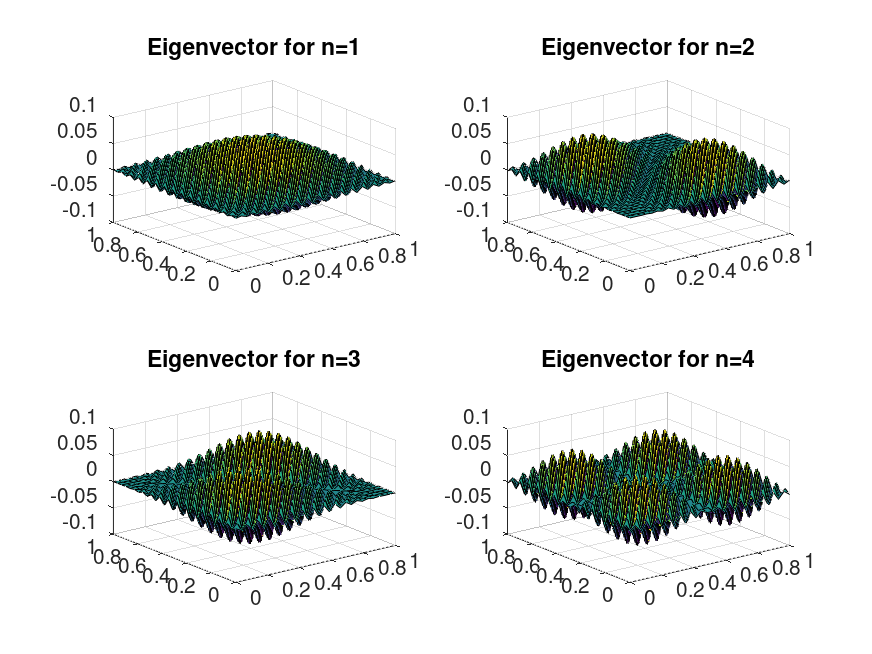
\includegraphics[width=0.75\textwidth]{problem_1c_eigenvectors.png}
        \caption{Eigenvectors for 2D eigenvalue Dirichlet BVP}
    \end{figure}
\end{solution}